\documentclass[11pt,a4paper]{article}

\usepackage[T1]{fontenc}
\usepackage[utf8]{inputenc}
\usepackage{lmodern}
\usepackage{microtype}
\usepackage[a4paper,margin=20mm]{geometry}
\usepackage{amsmath,amssymb,amsthm,mathtools,bm}
\usepackage{booktabs,longtable,tabularx,array,multirow}
\usepackage{calc}
\usepackage{enumitem}
\usepackage{xcolor}
\usepackage{hyperref}
\usepackage{setspace}
\usepackage{fancyhdr}
\usepackage{graphicx}
\usepackage{caption}
\usepackage{float}
\usepackage{placeins}
\usepackage{tikz}
\usetikzlibrary{arrows.meta,calc,positioning,shapes.geometric,fit}

\definecolor{navy}{HTML}{17365D}
\definecolor{slate}{HTML}{394B59}
\definecolor{lightblue}{HTML}{EAF1F8}
\definecolor{lightgray}{HTML}{F3F5F7}
\definecolor{lightgreen}{HTML}{EAF6EE}
\definecolor{lightred}{HTML}{FBECEC}
\definecolor{amber}{HTML}{FFF3D6}
\definecolor{deepgreen}{HTML}{1E6B3A}
\definecolor{deepred}{HTML}{9B1C1C}
\definecolor{deepamber}{HTML}{8A5B00}
\definecolor{purple}{HTML}{5B3F8C}

\hypersetup{
  colorlinks=true,
  linkcolor=navy,
  citecolor=navy,
  urlcolor=navy,
  pdftitle={Environmental Non-Screening and Finite-Size Stabilization in Z6 QCD Chronometry},
  pdfsubject={Nonlinear Earth, Sun and laboratory profiles for the protected ratio mode}
}

\setstretch{1.045}
\setlength{\parindent}{0pt}
\setlength{\parskip}{0.50em}
\setlist[itemize]{leftmargin=1.55em,itemsep=0.16em,topsep=0.20em}
\setlist[enumerate]{leftmargin=1.75em,itemsep=0.16em,topsep=0.20em}
\captionsetup{font=small,labelfont=bf}
\providecommand{\tightlist}{\setlength{\itemsep}{0pt}\setlength{\parskip}{0pt}}

\pagestyle{fancy}
\fancyhf{}
\fancyhead[L]{\small\color{slate}Environmental $Z_6$ QCD Chronometry}
\fancyhead[R]{\small\color{slate}Technical note v0.7}
\fancyfoot[C]{\thepage}
\renewcommand{\headrulewidth}{0.3pt}

\newtheorem{theorem}{Theorem}[section]
\newtheorem{proposition}[theorem]{Proposition}
\newtheorem{corollary}[theorem]{Corollary}
\newtheorem{criterion}[theorem]{Acceptance criterion}
\newcolumntype{L}[1]{>{\raggedright\arraybackslash}p{#1}}
\newcolumntype{Y}{>{\raggedright\arraybackslash}X}

\newcommand{\statusbox}[2]{%
\begin{center}
\fcolorbox{#1}{#1!7}{\parbox{0.92\textwidth}{#2}}
\end{center}}

\begin{document}
\pagenumbering{gobble}

\begin{titlepage}
\thispagestyle{empty}
\vspace*{7mm}

{\color{navy}\rule{\textwidth}{1.2pt}}
\vspace{7mm}

{\fontsize{20}{24}\selectfont\bfseries\color{navy} Environmental Non-Screening and\\ Finite-Size Stabilization in\\ $Z_6$ QCD Chronometry\par}
\vspace{3mm}
{\Large Nonlinear Earth, Sun and laboratory profiles for the protected ratio mode\par}

\vspace{9mm}

\begin{center}
\begin{minipage}{0.93\textwidth}
\colorbox{lightgreen}{\parbox{0.96\textwidth}{
\textbf{Main conclusion.} For the v0.6 benchmark, exact nonlinear spherical solutions for Earth, the Sun and a 5 cm tungsten source remain on the unscreened thick-shell branch. The largest nonlinear correction is $1.41\times10^{-18}$. Although the solar core lies above the spinodal density of the corresponding infinite homogeneous medium, the strongest solar sub-region reaches only
\[
\frac{q_{\max}}{q_{\rm conv}}=1.02\times10^{-12}.
\]
Finite-size gradient energy prevents phase conversion. The visible $2/27$ QCD response therefore survives without environmental charge suppression; the benchmark signal is small because the coupling is small, not because matter screens it.
}}
\end{minipage}
\end{center}

\vfill

\begin{tabularx}{\textwidth}{@{}p{0.22\textwidth}X@{}}
Document status: & Technical research note; not peer reviewed \\
Version: & 0.7 \\
Date: & 16 August 2026 \\
Benchmark: & $M=10$ TeV, $f_a=M_{\rm P}$, $\epsilon=10^{-6}$, $m_a=3.80\times10^{-21}$ eV \\
Methods: & Exact nonlinear spherical boundary-value solutions, local-spinodal analysis, exterior-capacity bound and numerical verification \\
Principal result: & No thin shell and no matter-driven adjacent-phase core for Earth, Sun or laboratory sources
\end{tabularx}

\vspace{7mm}
{\color{navy}\rule{\textwidth}{1.2pt}}
\end{titlepage}

\pagenumbering{roman}

\begin{abstract}
We solve the nonlinear finite-density field equation of the $Z_6$-protected QCD chronometry model for Earth, solar and laboratory sources. Visible matter contributes through the threshold law $m_A(x)/m_A(\pi/2)=[1-\epsilon\cos x]^{p_A}$, with $p_A\le 2/27$. The local homogeneous potential has a spinodal at $t_*=0.1727234$, corresponding to $46.25\,\mathrm{g\,cm^{-3}}$ for the benchmark. The solar core exceeds this density, so an infinite medium would lose the metastable branch connected to $x=\pi/2$. A finite body, however, must also pay gradient energy. We derive a necessary spherical phase-conversion condition $q(R_c)>q_{\rm conv}=0.633135$, where $q(R_c)=M(<R_c)p\epsilon/(4\pi f_a^2R_c)$. The largest value in the modeled Sun is $6.43\times10^{-13}$. Exact adaptive boundary-value solutions give screening factors equal to unity to numerical precision for all three sources. The protected $2/27$ QCD response is therefore not screened, while source-induced clock shifts remain small because $d_g=7.41\times10^{-8}$. We identify cosmological vacuum/domain selection, rather than terrestrial or solar screening, as the next decisive problem.
\end{abstract}

\setcounter{tocdepth}{1}
\begingroup
\small
\setlength{\parskip}{0pt}
\tableofcontents
\endgroup
\clearpage
\pagenumbering{arabic}
\section{Main conclusion}\label{main-conclusion}

For the v0.6 benchmark

\[
M=10\,\mathrm{TeV},\qquad f_a=M_{\rm P},\qquad \epsilon=10^{-6},
\]

with

\[
m_a=3.79715\times10^{-21}\,\mathrm{eV},\qquad
\lambda_a=m_a^{-1}=347.38\,\mathrm{AU},
\]

the exact nonlinear spherical field equation was solved for an Earth
density model, a centrally concentrated solar model, and a uniform 5 cm
tungsten sphere. All three bodies are on the \textbf{unscreened
thick-shell branch}:

\[
\mathcal F_{\rm screen}=1
\]

to the numerical accuracy of the solve. The largest bounded nonlinear
correction is \(1.41\times10^{-18}\) for the Sun.

The solar core is locally dense enough that an infinite homogeneous
medium would remove the metastable \(x=\pi/2\) minimum. Nevertheless,
the Sun cannot move the field into the adjacent phase. Its strongest
concentric sub-region has scalar compactness only

\[
\frac{q_{\max}}{q_{\rm conv}}=1.02\times10^{-12}.
\]

The finite-size gradient cost overwhelms the local matter preference.
Thus the finite-density effect does \textbf{not} screen the visible
\(2/27\) QCD threshold response into oblivion. It also does not amplify
it: the benchmark remains weak because its unscreened coupling is small.



\section{Model and environmental
coupling}\label{model-and-environmental-coupling}

Let

\[
x\equiv\frac{a}{f_a}
\]

be the compact ratio mode. For the protected \(Z_6\) construction, take
the vacuum potential

\[
V_{Z_6}(x)=V_0\left(1+\cos 6x\right),
\qquad
V_0=\frac{m_a^2f_a^2}{36}.
\]

Choose the asymptotic vacuum

\[
x_\infty=\frac{\pi}{2}.
\]

The visible vectorlike threshold gives, at leading one-loop order,

\[
\frac{\Lambda_3(x)}{\Lambda_3(x_\infty)}
=
\left(1-\epsilon\cos x\right)^{2/27}.
\]

For a macroscopic body \(A\), write the scalar-dependent mass as

\[
A_A(x)
\equiv
\frac{m_A(x)}{m_A(x_\infty)}
=
\left(1-\epsilon\cos x\right)^{p_A},
\]

where

\[
p_A=\frac{2}{27}Q_{\Lambda,A}.
\]

Here \(Q_{\Lambda,A}\) is the fraction of the body's logarithmic mass
response carried by the low-energy QCD scale. The calculations use

\[
p\equiv\frac{2}{27},
\]

which is a conservative upper-envelope approximation
\(Q_{\Lambda,A}=1\). Nuclear and electromagnetic corrections generally
reduce the effective macroscopic charge and therefore reduce screening
relative to this benchmark.

For conserved nonrelativistic rest density \(\rho_{A*}(\mathbf x)\), the
effective potential is

\[
V_{\rm eff}(x,\mathbf x)
=
V_0(1+\cos 6x)
+
\sum_A\rho_{A*}(\mathbf x)A_A(x).
\]

The static equation is

\[
\boxed{
\nabla^2x
=
-\frac{m_a^2}{6}\sin 6x
+
\sum_A\frac{\rho_{A*}}{f_a^2}
 p_A\epsilon\sin x
\left(1-\epsilon\cos x\right)^{p_A-1}.
}
\]

Boundary conditions for an isolated spherical source are

\[
x'(0)=0,
\qquad
x(r\rightarrow\infty)=x_\infty.
\]

This equation is nonlinear in both the periodic vacuum force and the
matter coupling. No thin-shell or linear-response assumption is used in
the numerical solution.



\section{Dimensionless spherical
problem}\label{dimensionless-spherical-problem}

For a source of mass \(M\), radius \(R\), and density profile
\(\rho(r)\), define

\[
s=\frac rR,
\qquad
\mu=m_aR,
\]

and the normalized density shape

\[
D(s)=\frac{4\pi R^3\rho(Rs)}{M},
\qquad
\int_0^1D(s)s^2\,ds=1.
\]

The source strength is

\[
\boxed{
q_0
=
\frac{Mp\epsilon}{4\pi f_a^2R}.
}
\]

Using \(G=(8\pi M_{\rm P}^2)^{-1}\), this can be written as

\[
\boxed{
q_0
=
2p\epsilon
\left(\frac{M_{\rm P}}{f_a}\right)^2
\Phi_N,
\qquad
\Phi_N=\frac{GM}{Rc^2}.
}
\]

Let

\[
x=x_\infty+q_0u(s).
\]

Inside the source, the exact scaled equation becomes

\[
\boxed{
 u''+\frac2s u'
=
\mu^2u\,\operatorname{sinc}(6q_0u)
+
D(s)\cos(q_0u)
\left[1+\epsilon\sin(q_0u)\right]^{p-1}.
}
\]

Outside, the field approaches the Yukawa form

\[
x-x_\infty
=
-q_{\rm eff}\frac{R}{r}e^{-m_a(r-R)}.
\]

At the surface this gives the exact Robin condition

\[
u'(1)+(1+\mu)u(1)=0.
\]

The linearized problem is

\[
 u''+\frac2s u'=\mu^2u+D(s).
\]

The screening factor used below is

\[
\boxed{
\mathcal F_{\rm screen}
=
\frac{u_{\rm nonlinear}(1)}{u_{\rm linear}(1)}.
}
\]

A value near one is unscreened. A thin shell would give a substantially
smaller magnitude.



\section{Homogeneous-medium
analysis}\label{homogeneous-medium-analysis}

A local homogeneous potential is useful but, by itself, can be badly
misleading for finite objects.

Define

\[
t
=
\frac{\rho p\epsilon}{m_a^2f_a^2}.
\]

For \(\epsilon\ll1\),

\[
\frac{V_{\rm eff}(x)-V_{\rm eff}(\pi/2)}{V_0}
=
1+\cos6x-36t\cos x+O(\epsilon).
\]

The stationary condition is

\[
\sin6x=6t\sin x.
\]

\subsection{Matter selects an adjacent vacuum
globally}\label{matter-selects-an-adjacent-vacuum-globally}

The vacuum has six degenerate minima. At any positive visible-matter
density,

\[
A(\pi/6)<A(\pi/2),
\]

so matter makes the adjacent minimum near \(x=\pi/6\) globally lower.
This does not imply that a finite body can move the field there: it says
only which phase an infinite homogeneous medium would prefer.

\subsection{Exact local spinodal}\label{exact-local-spinodal}

The metastable branch connected to \(x=\pi/2\) exists while

\[
6t
\le
\max_{x\in[\pi/3,\pi/2]}
\frac{\sin6x}{\sin x}.
\]

Writing \(c=\cos x\),

\[
\frac{\sin6x}{\sin x}
=32c^5-32c^3+6c.
\]

The relevant maximum occurs at

\[
\cos^2x_*
=
\frac{6-\sqrt{21}}{20},
\]

and gives

\[
D_*=1.036340417661276,
\qquad
\boxed{t_*=\frac{D_*}{6}=0.172723402943546.}
\]

For the benchmark,

\[
\rho_c
\equiv
\frac{m_a^2f_a^2}{p\epsilon}
=267.767\,\mathrm{g\,cm^{-3}},
\]

and hence

\[
\boxed{
\rho_{\rm spinodal}=t_*\rho_c
=46.2497\,\mathrm{g\,cm^{-3}}.
}
\]

Earth and tungsten stay below this local spinodal. The central solar
density in the adopted profile is about \(150\,\mathrm{g\,cm^{-3}}\), so
the solar core lies above it. The next section explains why this still
does not produce a screened or phase-converted Sun.




\begin{figure}[H]
\centering
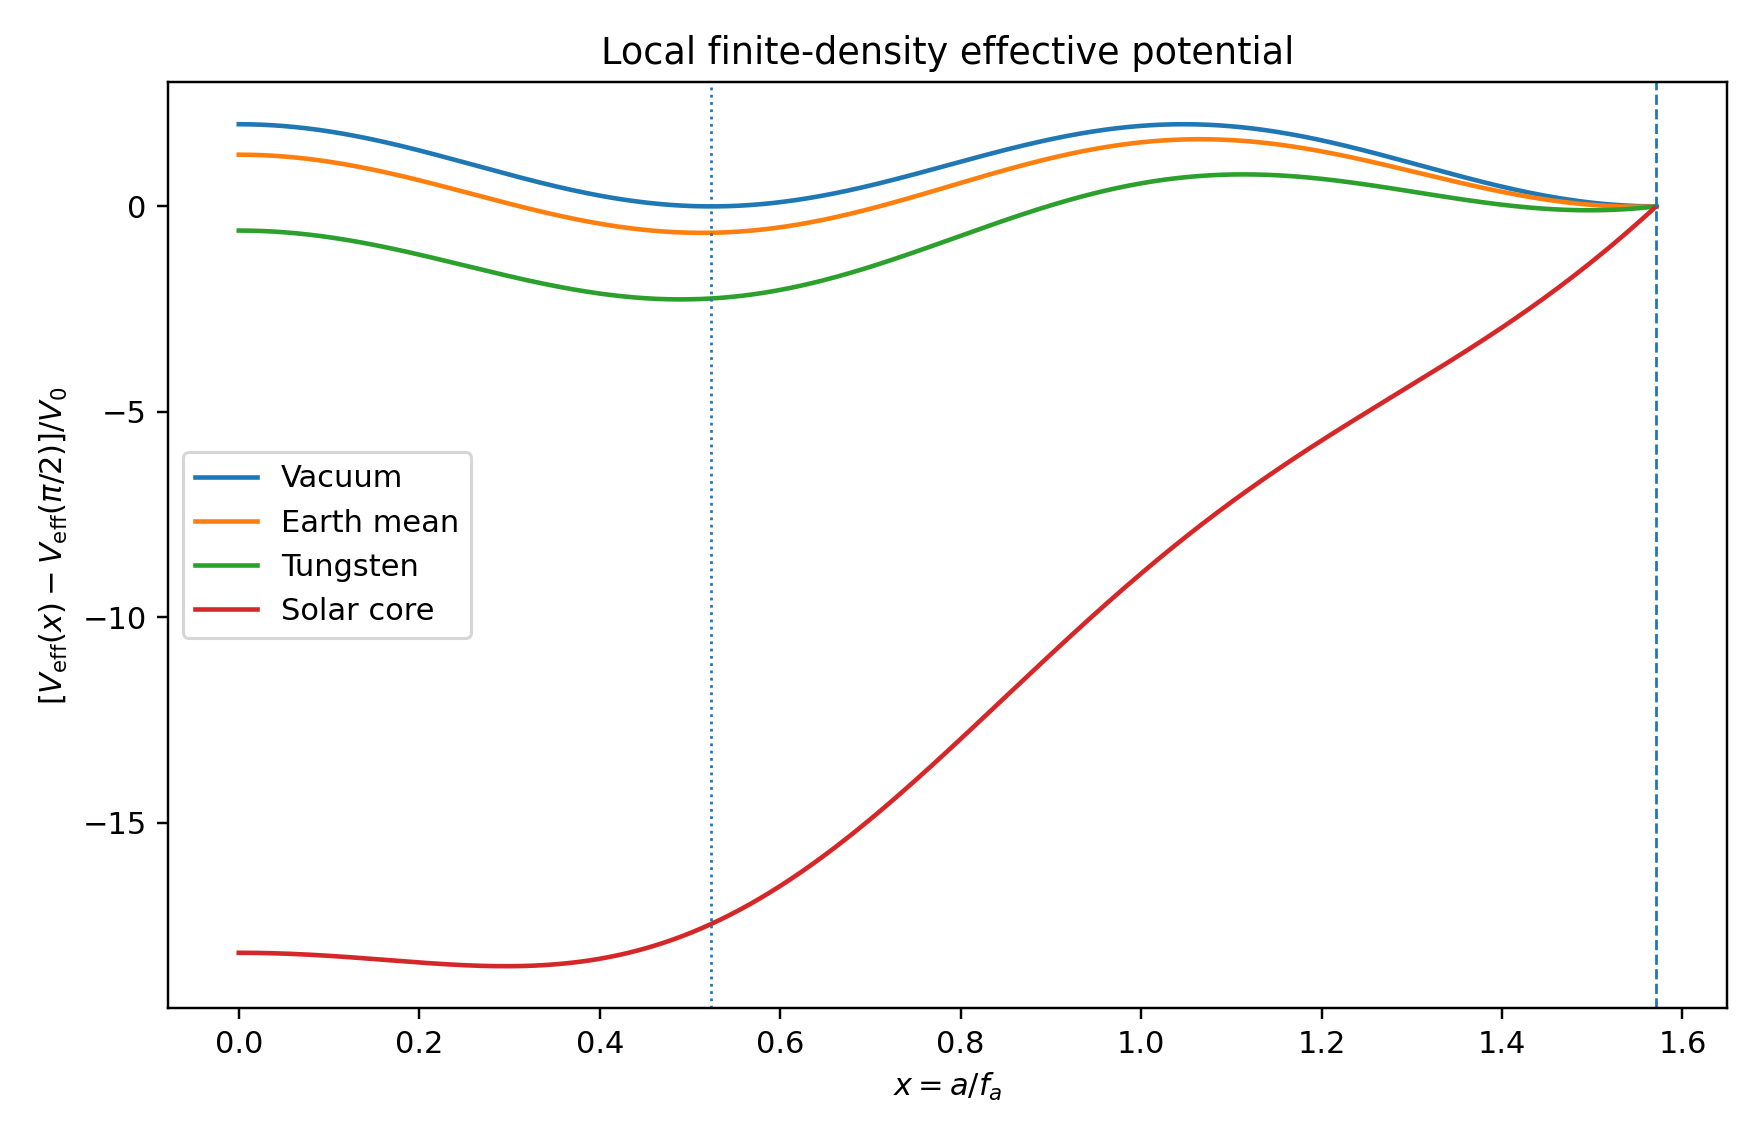
\includegraphics[width=0.92\textwidth]{environmental_effective_potential_v0_7.png}
\caption{Local homogeneous effective potentials. Visible matter tilts the sixfold vacuum toward the adjacent phase. The solar-core density removes the local branch connected to $x=\pi/2$ in the infinite-medium approximation; this does not imply that a finite Sun can realize that phase.}
\label{fig:local-potential}
\end{figure}

\section{Finite-size phase-conversion
bound}\label{finite-size-phase-conversion-bound}

Let

\[
\Delta x
=
\frac\pi2-\frac\pi6
=
\frac\pi3
\]

be the excursion from the asymptotic vacuum to the adjacent
matter-preferred phase.

The maximum rest-energy gain if a spherical source of mass \(M\)
converts completely is

\[
\Delta E_{\rm matter}
=
M\Delta A,
\]

where

\[
\Delta A
=
1-
\left(1-\frac{\sqrt3}{2}\epsilon\right)^p.
\]

Define

\[
C_\epsilon
=
\frac{\Delta A}{p\epsilon}
\longrightarrow
\frac{\sqrt3}{2}
\quad(\epsilon\rightarrow0).
\]

Then

\[
\Delta E_{\rm matter}
=
4\pi f_a^2Rq_0C_\epsilon.
\]

\subsection{Proposition: exterior-capacity lower
bound}\label{proposition-exterior-capacity-lower-bound}

If the field reaches the adjacent phase throughout a spherical core of
radius \(R_c\) and returns to \(x_\infty\) outside it, its exterior
gradient energy satisfies

\[
\boxed{
E_{\rm grad,out}
\ge
2\pi f_a^2R_c(\Delta x)^2.
}
\]

The minimum is attained, in the massless limit, by the harmonic profile

\[
\delta x(r)=-\Delta x\frac{R_c}{r}.
\]

The positive vacuum potential and a nonzero scalar mass can only
increase the required energy.

For a converted core, define

\[
q(R_c)
=
\frac{M(<R_c)p\epsilon}{4\pi f_a^2R_c}.
\]

A necessary condition for conversion is therefore

\[
4\pi f_a^2R_c q(R_c)C_\epsilon
>
2\pi f_a^2R_c(\Delta x)^2,
\]

or

\[
\boxed{
q(R_c)>q_{\rm conv}
\equiv
\frac{(\Delta x)^2}{2C_\epsilon}.
}
\]

For the benchmark,

\[
\boxed{q_{\rm conv}=0.633135.}
\]

This is the decisive finite-size criterion. The local spinodal depends
on density; actual conversion depends on integrated scalar compactness.

\subsection{Corollary: no converted phase outside a horizon for the
benchmark
class}\label{corollary-no-converted-phase-outside-a-horizon-for-the-benchmark-class}

For any concentric region with Newtonian compactness

\[
\Phi(R_c)=\frac{GM(<R_c)}{R_cc^2}<\frac12,
\]

one has

\[
q(R_c)
=
2p\epsilon
\left(\frac{M_{\rm P}}{f_a}\right)^2
\Phi(R_c).
\]

Therefore, if

\[
f_a\ge M_{\rm P},
\qquad
0<\epsilon\le1,
\qquad
p\le\frac{2}{27},
\]

then

\[
q(R_c)<p\le\frac{2}{27}=0.0741<q_{\rm conv}.
\]

Under these assumptions, no nonsingular spherical material region can
fully convert to the adjacent phase. The benchmark with
\(\epsilon=10^{-6}\) lies vastly deeper in the non-conversion regime.

This theorem does not exclude every possible nonlinear profile,
topological defect, cosmological domain history, or highly nonspherical
configuration. It does exclude the proposed matter-driven
adjacent-vacuum core for ordinary spherical bodies in the stated
parameter class.



\section{Why there is no thin
shell}\label{why-there-is-no-thin-shell}

Chameleon screening requires the field to settle near a
density-dependent interior minimum over most of a body, with only a thin
transition region contributing to the exterior charge. A standard
necessary indicator is

\[
m_{\rm eff,in}R\gg1.
\]

In the present model the relevant curvature scale remains of order
\(m_a\) throughout the branch explored by Earth, the Sun, and the
laboratory source. Their size parameters are

\[
\mu_{\oplus}=1.23\times10^{-7},
\qquad
\mu_\odot=1.34\times10^{-5},
\qquad
\mu_{\rm lab}=9.62\times10^{-16}.
\]

All satisfy

\[
\mu\ll1.
\]

The source is therefore much smaller than the field's response length.
The field cannot track the local minimum point by point; it responds to
the integrated source in the ordinary thick-shell regime.

The finite-density tilt may be large compared with the tiny vacuum
barrier in a hypothetical infinite medium, yet the body remains far too
small and too weakly compact to pay the spatial gradient cost. This is
the key distinction:

\[
\boxed{
\text{local phase preference}\neq\text{finite-body field realization}.
}
\]



\section{Numerical method}\label{numerical-method}

The exact spherical boundary-value problem was solved with an adaptive
collocation method.

The scaled variable \(u=(x-x_\infty)/q_0\) avoids loss of precision,
since the physical excursions are as small as \(10^{-32}\) for the
laboratory benchmark. The exterior domain is represented exactly through
the Robin condition at \(r=R\).

Three density profiles were used:

\begin{enumerate}
\def\labelenumi{\arabic{enumi}.}
\tightlist
\item
  \textbf{Earth:} a smoothed PREM-inspired four-layer profile with
  inner-core, outer-core, mantle, and crust densities, normalized to a
  mean density of \(5514\,\mathrm{kg\,m^{-3}}\).
\item
  \textbf{Sun:} an analytic centrally concentrated profile
  \(\rho(r)=\rho_c(1-r/R)^n\) with \(\rho_c=150\,\mathrm{g\,cm^{-3}}\)
  and exponent chosen to reproduce the mean density
  \(1408\,\mathrm{kg\,m^{-3}}\).
\item
  \textbf{Laboratory source:} a uniform tungsten sphere of radius
  \(5\,\mathrm{cm}\) and density \(19.25\,\mathrm{g\,cm^{-3}}\).
\end{enumerate}

The solver independently computes the linear and nonlinear profiles. The
nonlinear source terms are retained exactly. Convergence, normalization,
asymptotic matching, field-mass conversion, spinodal algebra, and
compactness identities are checked in the accompanying verification
script.



\section{Results}\label{results}

\begingroup\scriptsize
\begin{longtable}[]{@{}
  >{\raggedright\arraybackslash}p{(\columnwidth - 12\tabcolsep) * \real{0.1111}}
  >{\raggedleft\arraybackslash}p{(\columnwidth - 12\tabcolsep) * \real{0.1481}}
  >{\raggedleft\arraybackslash}p{(\columnwidth - 12\tabcolsep) * \real{0.1481}}
  >{\raggedleft\arraybackslash}p{(\columnwidth - 12\tabcolsep) * \real{0.1481}}
  >{\raggedleft\arraybackslash}p{(\columnwidth - 12\tabcolsep) * \real{0.1481}}
  >{\raggedleft\arraybackslash}p{(\columnwidth - 12\tabcolsep) * \real{0.1481}}
  >{\raggedleft\arraybackslash}p{(\columnwidth - 12\tabcolsep) * \real{0.1481}}@{}}
\toprule\noalign{}
\begin{minipage}[b]{\linewidth}\raggedright
Source
\end{minipage} & \begin{minipage}[b]{\linewidth}\raggedleft
\(\mu=m_aR\)
\end{minipage} & \begin{minipage}[b]{\linewidth}\raggedleft
\(q_0\)
\end{minipage} & \begin{minipage}[b]{\linewidth}\raggedleft
\(q_{\max}/q_{\rm conv}\)
\end{minipage} & \begin{minipage}[b]{\linewidth}\raggedleft
\(\delta x_c\)
\end{minipage} & \begin{minipage}[b]{\linewidth}\raggedleft
\(\delta x_R\)
\end{minipage} & \begin{minipage}[b]{\linewidth}\raggedleft
\(\mathcal F_{\rm scr}\)
\end{minipage} \\
\midrule\noalign{}
\endhead
\bottomrule\noalign{}
\endlastfoot
Earth & \(1.226\times10^{-7}\) & \(1.032\times10^{-16}\) &
\(1.63\times10^{-16}\) & \(-1.832\times10^{-16}\) &
\(-1.032\times10^{-16}\) & \(1.000000\) \\
Sun & \(1.339\times10^{-5}\) & \(3.145\times10^{-13}\) &
\(1.02\times10^{-12}\) & \(-1.518\times10^{-12}\) &
\(-3.145\times10^{-13}\) & \(1.000000\) \\
W sphere, \(R=5\) cm & \(9.621\times10^{-16}\) & \(2.218\times10^{-32}\)
& \(3.50\times10^{-32}\) & \(-3.328\times10^{-32}\) &
\(-2.218\times10^{-32}\) & \(1.000000\) \\
\end{longtable}
\endgroup

The linear Yukawa surface form factors are

\[
\mathcal F_Y^{\oplus}=0.9999998774,
\]

\[
\mathcal F_Y^{\odot}=0.9999866128,
\]

\[
\mathcal F_Y^{\rm lab}=0.99999999999.
\]

The nonlinear corrections are bounded by

\[
1.70\times10^{-22}
\quad\text{(Earth)},
\]

\[
1.41\times10^{-18}
\quad\text{(Sun)},
\]

\[
3.08\times10^{-38}
\quad\text{(laboratory)}.
\]

Thus the source charges are not thin-shell suppressed.




\begin{figure}[H]
\centering
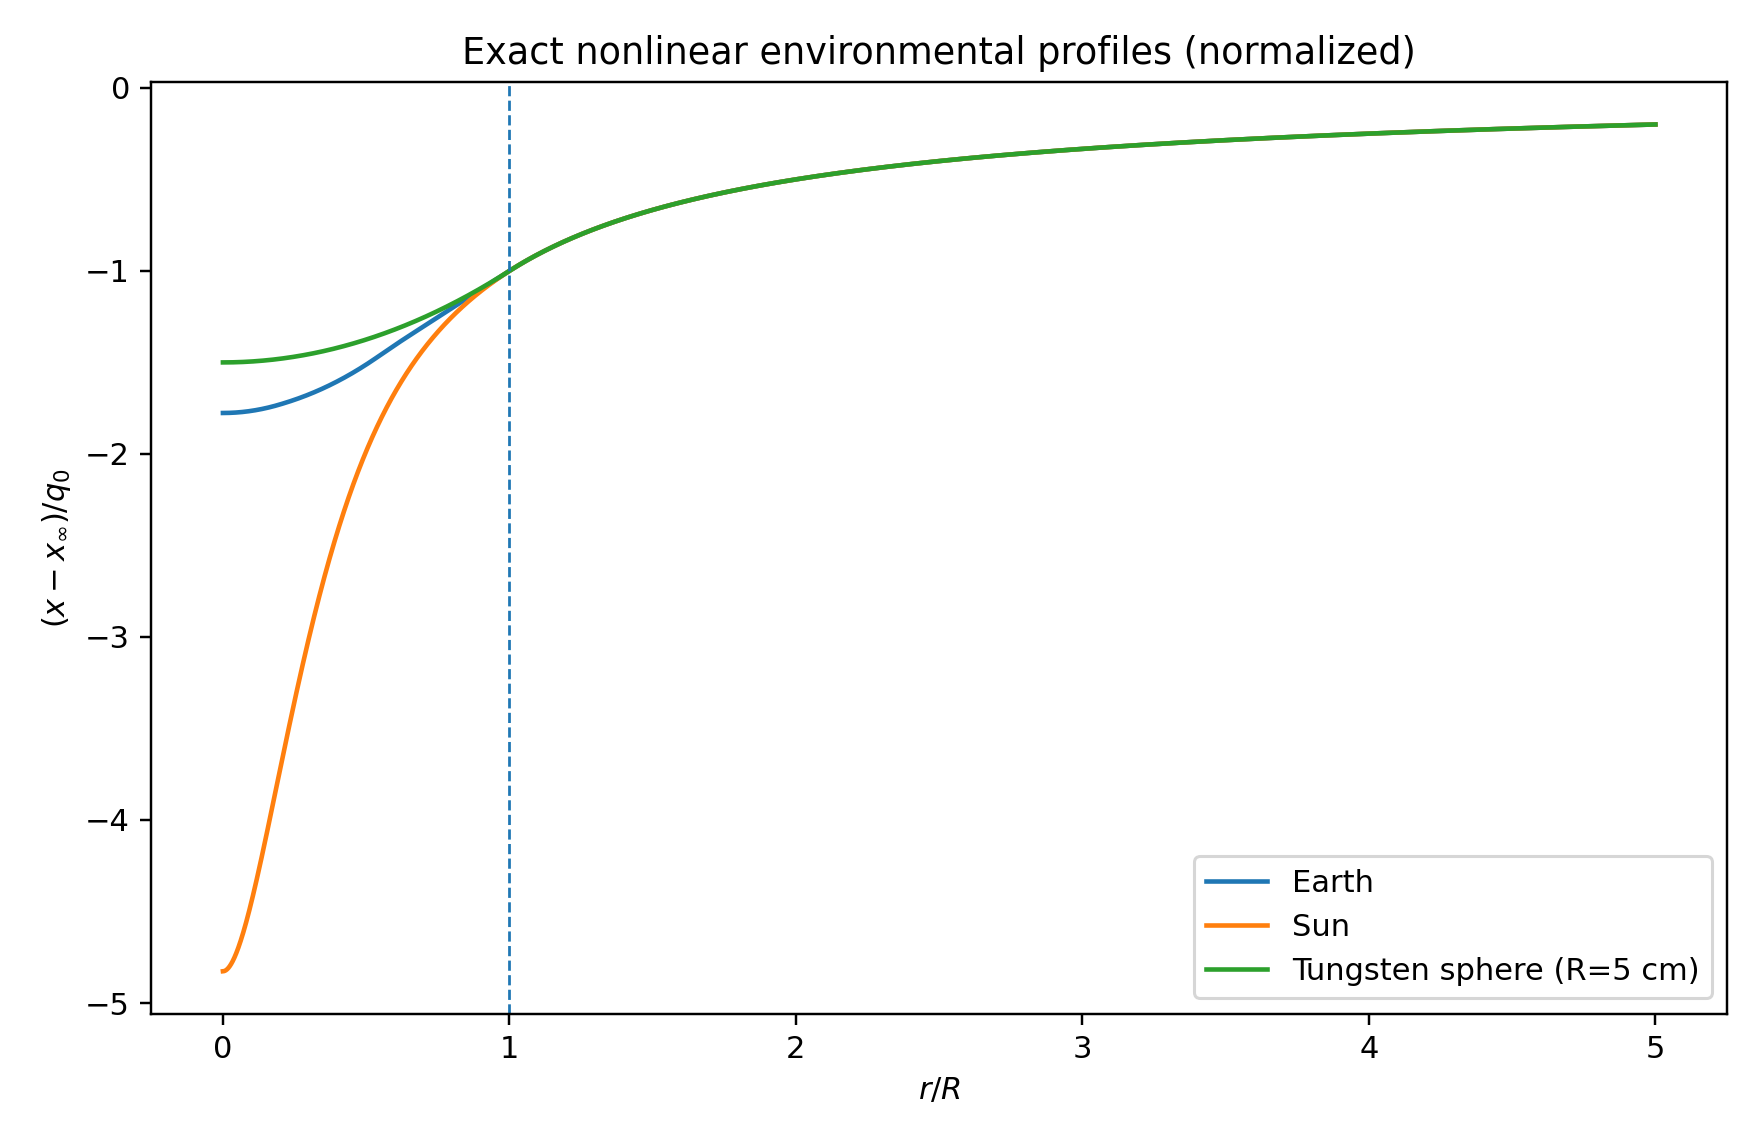
\includegraphics[width=0.94\textwidth]{environmental_profiles_v0_7.png}
\caption{Exact nonlinear environmental profiles normalized by the unscreened scalar compactness $q_0$. The dashed line is the source surface. The uniform sphere approaches the analytic massless values $u(0)=-3/2$ and $u(1)=-1$; central concentration deepens the interior solar and terrestrial profiles without suppressing their exterior charge.}
\label{fig:profiles}
\end{figure}

\section{The solar-core result}\label{the-solar-core-result}

The adopted solar profile exceeds the local spinodal density within

\[
R_c=0.1621R_\odot,
\]

containing approximately

\[
19.64\% 
\]

of the modeled solar mass.

For that patch,

\[
\bar t_c=0.2428>t_*,
\]

so an infinite homogeneous medium at the same mean density would not
retain the metastable branch connected to \(x=\pi/2\).

However,

\[
q_c=3.81\times10^{-13},
\]

and therefore

\[
\boxed{
\frac{q_c}{q_{\rm conv}}=6.02\times10^{-13}.
}
\]

Scanning all concentric solar sub-spheres gives the maximum

\[
q_{\max}=6.43\times10^{-13}
\]

at

\[
R_c\simeq0.368R_\odot,
\]

still only

\[
1.02\times10^{-12}
\]

of the necessary conversion compactness.

The exact nonlinear solution therefore stays continuously connected to
the asymptotic phase. The central excursion is only

\[
|x(0)-x_\infty|=1.52\times10^{-12}.
\]

The apparent solar-core instability was an artefact of applying an
infinite-medium effective potential without its gradient terms.




\begin{figure}[H]
\centering
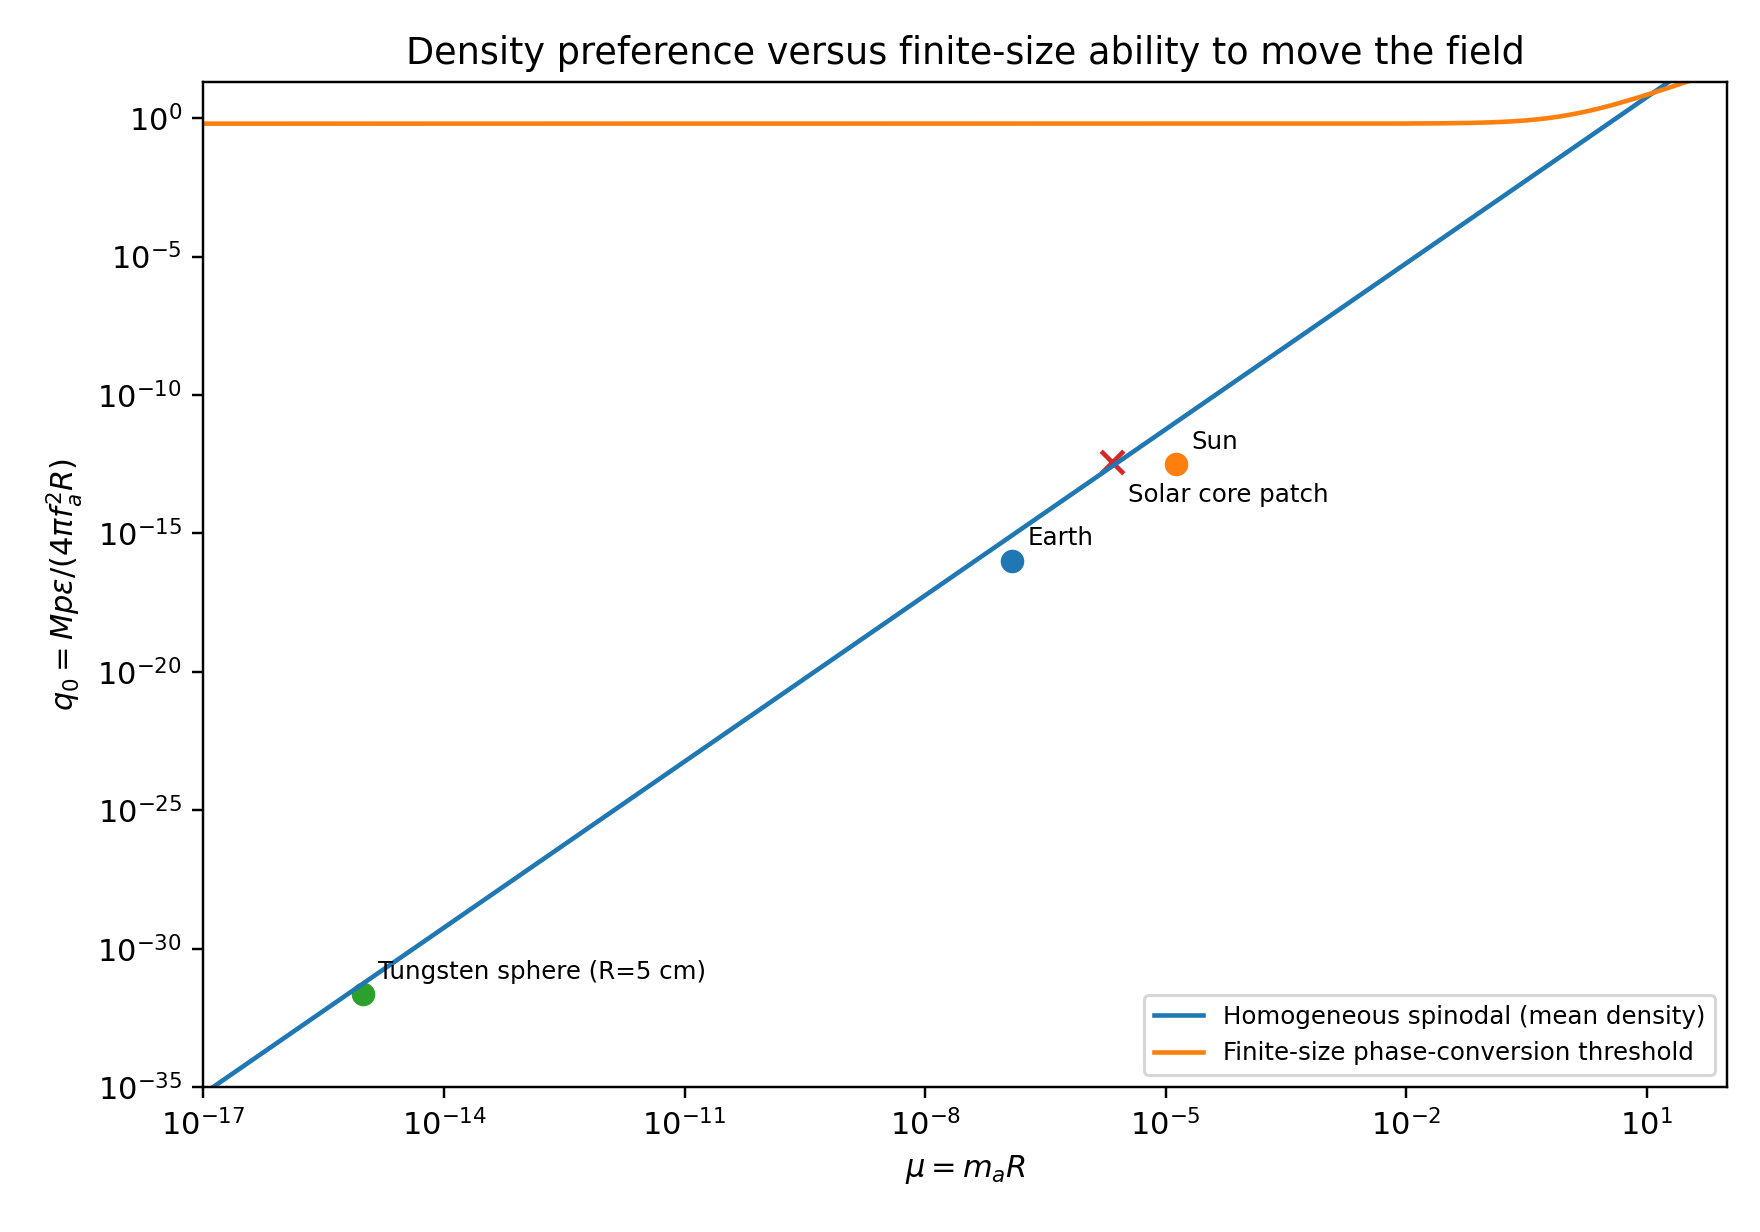
\includegraphics[width=0.92\textwidth]{environmental_screening_map_v0_7.png}
\caption{The blue curve marks the homogeneous spinodal inferred from mean density; the orange curve is the finite-size phase-conversion threshold. The solar-core patch lies above the local spinodal but roughly twelve orders of magnitude below the compactness required to move the field into the adjacent phase.}
\label{fig:screening-map}
\end{figure}

\section{Clock and fifth-force
signals}\label{clock-and-fifth-force-signals}

At \(x_\infty=\pi/2\), the visible QCD coupling is

\[
\boxed{
d_g
=
M_{\rm P}\frac{\partial}{\partial a}
\ln\frac{\Lambda_3}{\chi}
=
\frac{2}{27}\frac{M_{\rm P}}{f_a}\epsilon.
}
\]

For the benchmark,

\[
d_g=7.4074\times10^{-8}.
\]

For a clock-pair sensitivity combination
\(K_{AB}=\Delta K_\mu-\Delta K_q\), the source-induced ratio shift is

\[
\delta\ln\frac{\nu_A}{\nu_B}
=K_{AB}d_g\frac{f_a}{M_{\rm P}}\delta x.
\]

For \(|K_{AB}|=1\), the unscreened surface magnitudes are

\[
7.64\times10^{-24}
\quad\text{(Earth)},
\]

\[
2.33\times10^{-20}
\quad\text{(Sun)},
\]

\[
1.64\times10^{-39}
\quad\text{(5 cm tungsten sphere)}.
\]

At Earth's orbit, the solar field gives approximately

\[
|\delta x(1\,\mathrm{AU})|
=1.46\times10^{-15},
\]

and therefore

\[
\left|\delta\ln\frac{\nu_A}{\nu_B}\right|
\simeq
1.08\times10^{-22}|K_{AB}|.
\]

A simple eccentric-orbit estimate gives an annual modulation of order

\[
3.61\times10^{-24}|K_{AB}|.
\]

These values are not suppressed by environmental nonlinearities. They
are intrinsically small because the protected benchmark uses
\(\epsilon=10^{-6}\).

The unscreened universal scalar-force strength before composition
factors is approximately

\[
\frac{F_a}{F_N}\simeq2d_g^2
=1.10\times10^{-14}
\]

for separations short compared with \(\lambda_a\). Composition-dependent
free-fall signals are further weighted by differences of nuclear dilaton
charges.

The v0.5 clock--equivalence-principle consistency relation is therefore
retained without an environmental screening factor:

\[
\frac{\beta_{AB}}{\eta_{CD}}
=
-
\frac{\Delta K_\mu-\Delta K_q}
{\Delta Q'_{\widehat m}{}^{CD}}
\]

within the one-scalar, unscreened, pure-QCD approximation.



\section{Robustness and
limitations}\label{robustness-and-limitations}

\subsection{Composition}\label{composition}

Using \(p=2/27\) assumes the entire source mass scales with
\(\Lambda_3\). Real atoms contain electron, quark-mass, electromagnetic,
and nuclear-binding contributions. Replacing \(p\) with
species-dependent \(p_A\) changes the quantitative charge and
equivalence-principle response. Since the QCD fraction is below unity,
the benchmark choice generally overestimates the environmental source
strength.

\subsection{Solar model}\label{solar-model}

The analytic solar profile is not a precision standard-solar-model
table. It was chosen to reproduce the correct gross radius, mass, mean
density, and a representative central density while retaining a smooth
profile. The no-screening result has a margin of twelve orders of
magnitude in the conversion criterion, so realistic profile refinements
cannot reverse it.

\subsection{Pressure and
temperature}\label{pressure-and-temperature}

The environmental source for a relativistic scalar coupling is more
precisely the appropriate derivative of the matter free energy and, in
many frames, is related to the stress-energy trace. Earth, laboratory
matter, and most solar rest mass are nonrelativistic enough that
\(\rho A(x)\) captures the leading effect. Neutron stars and the early
Universe require an equation-of-state treatment.

\subsection{Higher-order QCD threshold
corrections}\label{higher-order-qcd-threshold-corrections}

The exponent \(2/27\) receives calculable perturbative matching
corrections. They alter \(p\) by relative \(O(\alpha_s)\) factors but do
not bridge the \(10^{12}\) gap to phase conversion.

\subsection{Geometry}\label{geometry}

The exact BVP calculations are spherical. The capacity argument
generalizes qualitatively to arbitrary shapes, but the numerical
threshold is shape-dependent through electrostatic capacity. Ordinary
laboratory geometries remain fantastically below the required scalar
compactness.

\subsection{Cosmology and domains}\label{cosmology-and-domains}

The fact that any positive homogeneous visible density energetically
selects an adjacent \(Z_6\) vacuum remains important for cosmological
history. A finite star cannot nucleate the phase, but an early
homogeneous Universe may move the field when Hubble friction,
temperature-dependent sector populations, and causal domain sizes are
included. Vacuum/domain selection is now a more serious issue than
terrestrial screening.

\subsection{Screening mechanisms not
included}\label{screening-mechanisms-not-included}

The calculation excludes additional derivative screening, nonlinear
kinetic terms, independent chameleon couplings, plasma-induced terms
from hidden-sector populations, and explicit \(Z_6\)-breaking operators.
Any ultraviolet completion must be re-evaluated if it introduces such
terms.



\section{Novelty boundary}\label{novelty-boundary}

Finite-density scalar potentials, density-dependent destabilization,
chameleon thin shells, and nonlinear spherical profile methods are
established subjects.

The candidate contribution here is narrower:

\begin{enumerate}
\def\labelenumi{\arabic{enumi}.}
\tightlist
\item
  the exact environmental equation for the protected visible \(2/27\)
  QCD threshold model;
\item
  the separation between the homogeneous spinodal and finite-size scalar
  compactness;
\item
  the capacity lower bound applied to adjacent \(Z_6\) phase conversion;
\item
  the result that the solar core can lie above the local spinodal while
  the full nonlinear Sun remains unscreened and unconverted by twelve
  orders of magnitude;
\item
  preservation of the chronometric clock--equivalence-principle
  consistency line without a screening factor.
\end{enumerate}

A complete priority claim would still require backward and forward
citation analysis across finite-density axion, symmetron, chameleon,
scalarization, and false-vacuum bubble literature.



\section{Acceptance matrix}\label{acceptance-matrix}

\begin{longtable}[]{@{}
  >{\raggedright\arraybackslash}p{(\columnwidth - 4\tabcolsep) * \real{0.3000}}
  >{\raggedleft\arraybackslash}p{(\columnwidth - 4\tabcolsep) * \real{0.4000}}
  >{\raggedright\arraybackslash}p{(\columnwidth - 4\tabcolsep) * \real{0.3000}}@{}}
\toprule\noalign{}
\begin{minipage}[b]{\linewidth}\raggedright
Requirement
\end{minipage} & \begin{minipage}[b]{\linewidth}\raggedleft
Verdict
\end{minipage} & \begin{minipage}[b]{\linewidth}\raggedright
Evidence
\end{minipage} \\
\midrule\noalign{}
\endhead
\bottomrule\noalign{}
\endlastfoot
Exact nonlinear environmental equation & \textbf{PASS} & Derived from
\(V_{Z_6}+\rho A(x)\) \\
Earth boundary-value solution & \textbf{PASS} & Adaptive nonlinear BVP
converged \\
Solar boundary-value solution & \textbf{PASS} & Adaptive nonlinear BVP
converged \\
Laboratory-source solution & \textbf{PASS} & Adaptive nonlinear BVP
converged \\
Thin-shell screening & \textbf{ABSENT} & \(m_{\rm eff}R\ll1\),
\(\mathcal F_{\rm screen}=1\) \\
Adjacent-phase conversion & \textbf{EXCLUDED for benchmark spherical
sources} & Capacity bound and \(q_{\max}/q_{\rm conv}\ll1\) \\
Solar-core local destabilization & \textbf{PRESENT in homogeneous
approximation} & \(\rho_{\rm core}>\rho_{\rm spinodal}\) \\
Solar-core actual conversion & \textbf{ABSENT} &
\(q_c/q_{\rm conv}=6.02\times10^{-13}\) \\
Visible \(2/27\) response & \textbf{PRESERVED} & No environmental charge
suppression \\
Observable benchmark clock signal & \textbf{NO} & Unscreened but
\(\lesssim10^{-20}\) at solar surface \\
Cosmological vacuum selection & \textbf{OPEN} & Requires
finite-temperature FRW evolution \\
Nonspherical and multi-body validation & \textbf{OPEN but unlikely to
alter benchmark verdict} & Huge compactness margin \\
Neutron-star treatment & \textbf{OPEN} & Requires relativistic EOS and
full GR \\
\end{longtable}



\section{Next decisive step}\label{next-decisive-step}

Environmental screening is not the bottleneck for the protected
benchmark. The next calculation should therefore combine two tasks:

\begin{enumerate}
\def\labelenumi{\arabic{enumi}.}
\tightlist
\item
  \textbf{Cosmological vacuum selection:} solve \[
  \ddot x+3H\dot x-\frac{\nabla^2x}{a_{\rm FRW}^2}
  =-\frac{1}{f_a^2}\frac{\partial V_{\rm eff}(x,T,\rho_k)}{\partial x}
  \] through reheating, replicated-sector decoupling, the QCD crossover,
  and matter domination to determine whether the Universe lands in the
  visible \(x_\infty=\pi/2\) branch without unacceptable walls or
  isocurvature.
\item
  \textbf{Observable-coupling optimization:} vary \((M,f_a,\epsilon,N)\)
  subject to radiative protection, fifth-force limits, clock limits,
  cosmology, and the no-conversion condition to determine the largest
  allowed nonzero chronometric shear.
\end{enumerate}

The environmental result is conceptually favourable:

\[
\boxed{
\text{the source remains visible to the field; it is the coupling, not screening, that limits the signal.}
}
\]



\section{References}\label{references}

\begin{enumerate}
\def\labelenumi{\arabic{enumi}.}
\tightlist
\item
  D. Cyncynates and O. Simon, \emph{Cosmology and Astrophysics of
  CP-Violating Axions}, arXiv:2408.02294.
\item
  J. Khoury and A. Weltman, \emph{Chameleon Fields: Awaiting Surprises
  for Tests of Gravity in Space}, arXiv:astro-ph/0309300.
\item
  T. Tamaki and S. Tsujikawa, \emph{Revisiting chameleon gravity:
  thin-shells and no-shells with appropriate boundary conditions},
  arXiv:0808.2284.
\item
  T. Damour and J. F. Donoghue, \emph{Equivalence Principle Violations
  and Couplings of a Light Dilaton}, arXiv:1007.2792.
\item
  P. Touboul et al., \emph{MICROSCOPE Mission: Final Results of the Test
  of the Equivalence Principle}, arXiv:2209.15487.
\item
  NASA/NSSDC, \emph{Earth Fact Sheet}.
\item
  NASA/GSFC, \emph{Sun Fact Sheet}.
\item
  Previous project note v0.6, \emph{Cyclic Discrete-Goldstone Protection
  of QCD Chronometric Shear}.
\end{enumerate}

\end{document}
